%! Author = Johannes Byle
%! Date = 8/30/2021

% Preamble
\documentclass[12pt]{article}
\title{Classical Mechanics Assignment \#1}
\author{Johannes Byle}

% Packages
\usepackage{amsmath}
\usepackage[margin=0.75in]{geometry}
\usepackage{lipsum}
\usepackage{braket}
\usepackage{tikz}
\usepackage{pgfplots}

% Document
\begin{document}
    \maketitle
    \begin{enumerate}
        \item
        \begin{enumerate}
            \item
            Starting with the forces, simplifying, and substituting variables:
            \begin{gather*}
                F_{\text{total}}=F_{\text{spring}}+F_{\text{damping}}+F_{\text{piston}}\\
                m\ddot{x}=-kx-m\nu\dot{x}+kX(t)\\
                \ddot{x}+\frac{k}{m}x+\nu\dot{x}=\frac{k}{m}(t)\\
                \ddot{x}+\nu\dot{x}+\omega_0^2 x=F_0(t)
            \end{gather*}
            \item
            Complementary solution:
            \begin{gather*}
                x(t)=e^{-\beta t}\left[A_1 e^{-i\sqrt{\omega_0^2-\beta^2}t}+A_2 e^{i\sqrt{\omega_0^2-\beta^2}t}\right]
            \end{gather*}
            Starting the particular solution by finding the derivatives of $X(t)$:
            \begin{gather*}
                X(t)=X_0 e^{\alpha t}\cos(\omega t+\delta)\\
                \dot{X}(t)=e^{\alpha t}X_0\left(\alpha\cos(\omega t+\delta)-\omega\sin(\omega t+\delta)\right)\\
                \ddot{X}(t)=X_0 e^{\alpha t} \left(\left(\alpha^2-\omega^2\right) \cos (\omega t+\delta)-2 \alpha \omega \sin (\omega t+\delta)\right)\\
            \end{gather*}
            Substituting back into equation:
            \begin{gather*}
                X_0 e^{\alpha t} \left(\left(\alpha^2-\omega^2\right) \cos (t \omega)-2 \alpha \omega \sin (t \omega)\right)+\\
                \nu e^{\alpha t}X_0\left(\alpha\cos(\omega t)-\omega\sin(\omega t)\right)+\\
                \omega_0^2 X_0 e^{\alpha t}\cos(\omega t)=\omega_0^2 e^{\alpha t}\cos(\omega t)\\
            \end{gather*}
            Solving for $\cos$ terms:
            \begin{gather*}
                X_0 e^{\alpha t}\left(\alpha^2-\omega^2\right)+\nu e^{\alpha t}X_0\alpha+\omega_0^2 X_0 e^{\alpha t}=\omega_0^2 e^{\alpha t}\\
                X_0\left[e^{\alpha t}\left(\alpha^2-\omega^2\right)+\nu e^{\alpha t}\alpha+\omega_0^2 e^{\alpha t}\right]=\omega_0^2 e^{\alpha t}\\
                X_0=\frac{\omega_0^2 e^{\alpha t}}{e^{\alpha t}\left(\alpha^2-\omega^2\right)+\nu e^{\alpha t}\alpha+\omega_0^2 e^{\alpha t}}\\
                X_0=\frac{\omega_0^2}{\alpha^2+\alpha\nu-\omega^2+\omega_0^2}
            \end{gather*}
            Particular solution:
            \begin{gather*}
                e^{-\beta t}\left[A_1 e^{-i\sqrt{\omega_0^2-\beta^2}t}+A_2 e^{i\sqrt{\omega_0^2-\beta^2}t}\right]=\frac{\omega_0^2}{\alpha^2+\alpha\nu-\omega^2+\omega_0^2}e^{\alpha t}\cos(\omega t)
            \end{gather*}
            \item
            At the steady state only the forcing function matters, and the amplitude of the steady state function will be maximum when:
            \begin{gather*}
                \omega=\sqrt{\alpha^2+\alpha\nu+\omega_0^2}=\omega_R
            \end{gather*}
            This does depend on the sign of $\alpha$, as if $\alpha$ is negative as $t\rightarrow\infty$ it will tend toward 0.
        \end{enumerate}
        \item
        \begin{enumerate}
            \item
            Assuming the "ripples" can be modeled by a sinusoidal function, the motion of the car can be described by the driven damped oscillator discussed in class.
            In this case the equation for the resonance frequency:
            \begin{gather*}
                \omega_r=\sqrt{\omega_0^2+2\beta^2}\\
                \frac{v}{x_\text{spacing}}=\sqrt{\omega_0^2+2\beta^2}\\
                v=x_\text{spacing}\sqrt{\omega_0^2+2\beta^2}\\
            \end{gather*}
            Since $\omega_0=\sqrt{\frac{k}{m}}$ and $\beta=\frac{b}{2m}$:
            \begin{gather*}
                \omega_r=\sqrt{\omega_0^2+2\beta^2}\\
                \frac{v}{x_\text{spacing}}=\sqrt{\omega_0^2+2\beta^2}\\
                v=x_\text{spacing}\sqrt{\frac{k}{m}+\frac{b^2}{4m^2}}\\
            \end{gather*}
            Plugging in some reasonable values we can check whether or not our equations make physical sense.
            I used the mass of my car $m=1565$ kg, and damping $b=2000$ N s/m and stiffness $k=22,000$ N/m parameters from a research paper.\footnote{https://journals.sagepub.com/doi/full/10.1177/1687814016648638 Analysis of suspension with variable stiffness and variable damping force for automotive applications}
            \begin{gather*}
                v=2\sqrt{\frac{22000}{1565}+\frac{2000^2}{4\cdot1565^2}}\approx7.6\text{ m/s}\approx17\text{ mph}\\
            \end{gather*}
            This is a reasonable number and the units make sense:
            \begin{gather*}
                v=m\sqrt{\frac{N}{m\cdot kg}+\frac{N^2\cdot s^2}{m^2\cdot kg^2}}\\
                v=m\sqrt{\frac{kg\cdot m}{m\cdot kg\cdot s^2}+\frac{kg^2\cdot m^2\cdot s^2}{m^2\cdot kg^2\cdot s^4}}\\
                v=m\sqrt{\frac{1}{s^2}+\frac{1}{s^2}}=\frac{m}{s}\\
            \end{gather*}
            \item
            So that the suspension doesn't fall apart I probably want a damping constant that only allows resonances at very high speeds, say above $100$ mph:
            \begin{gather*}
                \sqrt{4m^2\left(\frac{v^2}{x^2_\text{spacing}}-\frac{k}{m}\right)}=b\\
                \sqrt{4\cdot1565^2\left(\frac{45}{2}-\frac{22000}{1565}\right)}\approx 9100\text{ N s/m}\\
            \end{gather*}
        \end{enumerate}
        \item
        \begin{enumerate}
            \item
            Since $F=\frac{dU}{ds}$ the change in energy of the system is simply:
            \begin{gather*}
                m\ddot{x}=F=\dot{E}=-\left(x^2+\dot{x}^2-1\right)\dot{x}-x
            \end{gather*}
            \item
            By the definitions that $x=r\cos\theta$ and $\dot{x}=r\sin\theta$:
            \begin{gather*}
                r^2=r^2\cos^2\theta+r^2\sin^2\theta\\
                r^2=x^2+\dot{x}^2
            \end{gather*}
            Taking a time derivative and solving for $\ddot{x}$:
            \begin{gather*}
                \frac{d}{dt}(r^2)=\frac{d}{dt}\left(x^2+\dot{x}^2\right)\\
                2r\dot{r}=2x\dot{x}+2\dot{x}\ddot{x}\\
                \ddot{x}=\frac{r\dot{r}}{\dot{x}}-x
            \end{gather*}
            Substituting back in for $x$ and $\dot{x}$
            \begin{gather*}
                \ddot{x}=\frac{r\dot{r}}{r\sin\theta}-r\cos\theta\\
                \ddot{x}=\frac{\dot{r}}{\sin\theta}-r\cos\theta
            \end{gather*}
            Plugging it back into the original equation of motion:
            \begin{gather*}
                \frac{\dot{r}}{\sin\theta}-r\cos\theta=-\left(x^2+\dot{x}^2-1\right)\dot{x}-x\\
                \frac{\dot{r}}{\sin\theta}-r\cos\theta=-\left((r\cos\theta)^2+(r\sin\theta)^2-1\right)r\sin\theta-r\cos\theta\\
                \frac{\dot{r}}{\sin\theta}-r\cos\theta=-\left(r^2-1\right)r\sin\theta-r\cos\theta\\
                \dot{r}=-\left(r^2-1\right)r\sin^2\theta\\
                \dot{r}=r\left(1-r^2\right)\sin^2\theta
            \end{gather*}
            Repeating the same process to find $\dot{\theta}$:\\
            By the definitions that $x=r\cos\theta$ and $\dot{x}=r\sin\theta$:
            \begin{gather*}
                \frac{\dot{x}}{x}=\frac{r\sin\theta}{r\cos\theta}=\tan{\theta}
            \end{gather*}
            Taking a time derivative and solving for $\dot{\theta}$:
            \begin{gather*}
                \frac{d}{dt}\tan{\theta}=\frac{d}{dt}\frac{\dot{x}}{x}\\
                \frac{\dot{\theta}}{\cos^2{\theta}}=\frac{\ddot{x}}{x}-\frac{\dot{x}^2}{x^2}\\
                \dot{\theta}=\cos^2{\theta}\left(\frac{\ddot{x}}{x}-\frac{\dot{x}^2}{x^2}\right)
            \end{gather*}
            Substituting back in the equation of motion from part (a) for $\ddot{x}$:
            \begin{gather*}
                \dot{\theta}=\cos^2{\theta}\left(\frac{-\left(x^2+\dot{x}^2-1\right)\dot{x}-x}{x}-\frac{\dot{x}^2}{x^2}\right)
            \end{gather*}
            Substituting back in for $x$ and $\dot{x}$ and simplifying:
            \begin{gather*}
                \dot{\theta}=\cos^2{\theta}\left(\frac{-\left((r\cos\theta)^2+(r\sin\theta)^2-1\right)r\sin\theta-r\cos\theta}{r\cos\theta}-\frac{(r\sin\theta)^2}{(r\cos\theta)^2}\right)\\
                \dot{\theta}=\cos^2{\theta}\left(\frac{-\left(r^2-1\right)\sin\theta-\cos\theta}{\cos\theta}-\frac{\sin^2\theta}{\cos^2\theta}\right)\\
                \dot{\theta}=\cos^2{\theta}\left(\frac{-\left(r^2-1\right)\sin\theta}{\cos\theta}-\left[1+\frac{\sin^2\theta}{\cos^2\theta}\right]\right)\\
                \dot{\theta}=\cos^2{\theta}\left(\frac{-\left(r^2-1\right)\sin\theta}{\cos\theta}-\sec^2\theta\right)\\
                \dot{\theta}=-\left(r^2-1\right)\sin\theta\cos\theta-1\\
            \end{gather*}
            \item
            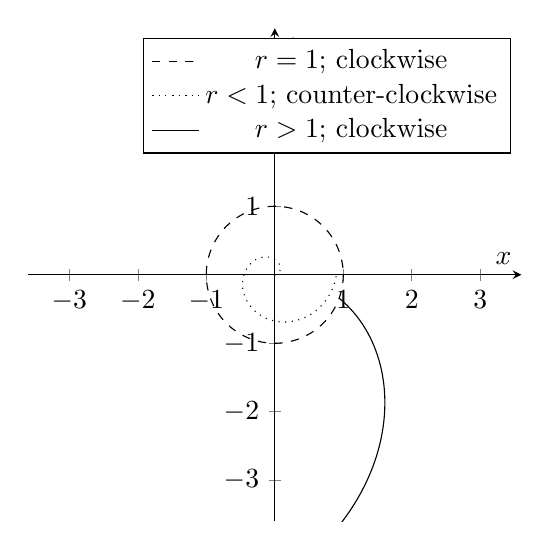
\begin{tikzpicture}
                \begin{axis}
                    [
                    axis lines=center,
                    axis equal image,
                    enlargelimits=true,
                    xlabel=$x$,
                    ylabel=$\dot{x}$,
                    width=0.75\linewidth,
                    xmin=-3,xmax=3,ymin=-3,ymax=3
                    ]
                    \addplot[
                        data cs=polar,
                        dashed,
                        domain=0:360,
                        samples=360,
                        smooth,
                        label=r,
                    ] (-1*x,1);
                    \addplot[
                        data cs=polar,
                        dotted,
                        domain=0:360,
                        samples=360,
                        smooth,
                        label=r,
                    ] (x,0.0025*x);
                    \addplot[
                        data cs=polar,
                        domain=20:100,
                        samples=360,
                        smooth,
                        label=r,
                    ] (-1*x,0.05*x);
                    \legend{$r=1;$ clockwise, $r<1;$ counter-clockwise, $r>1;$ clockwise};
                \end{axis}
            \end{tikzpicture}
        \end{enumerate}
    \end{enumerate}

\end{document}